\chapter{Scenario Series 6-2y}

This appendix presents simulation results from the 6-2y scenario series, which tests the impact of decreasing end-product prices in the agent network. 
We decrease all products prices proportionately (i.e., perfectly correlated price increase, relative to base values), and keep them constant for all 30 iterations. 

\section{Summary}
Table \ref{tab:scenario_list} below lists the scenarios in series 6-2x.
 
Base scenario s6-2x\_f1.0 is identical to s6-1\_p30a01, and simulates a basic bilevel scenario with default prices (i.e., scaling factor 1.0).
We tested scaling factors of 0.90 and 0.85. 
Profit is reduced significantly in the 0.90 scenario, however harvest levels are minimally impacted.
Hardwood price drops below the break-even point for the 0.85 scenario, which causes upper bound on the hardwood log consumption in the bilevel algorithm to drop suddenly to 0. 
This implies that agent softwood procurement must be limited to true pure softwood stands (i.e., absolutely no hardwood content in the yield curve model at harvest age). 
True pure softwood stands are quite rare in our dataset, so softwood log consumption drops to a very low level (approximately 1\% of base scenario fibre consumption).
Simulation results for scenarios testing factors less than 0.85 were omitted, as harvest drops to 0 for both hardwood and softwood.

\begin{table}
  \centering
  \begin{tabular}{lll}
    \hline
    Scenario ID & Figure Reference & Description \\
    \hline
    6-2y\_f1.00 & \ref{fig:s6-2y_test100} & Control scenario (same as s6-1\_p30a01). \\
    6-2y\_f0.90 & \ref{fig:s6-2y_test090} & Prices scaled by factor of 0.90 \\
    6-2y\_f0.85 & \ref{fig:s6-2y_test085} & Prices scaled by factor of 0.85 \\
    % 6-2y\_f5.3 & \ref{fig:s6-2y_test70} & Prices scaled by factor of 0.7 \\
    % 6-2y\_f4.6 & \ref{fig:s6-2y_test60} & Prices scaled by factor of 0.6 \\
    % 6-2y\_f4.0 & \ref{fig:s6-2y_test50} & Prices scaled by factor of 0.5 \\
    % 6-2y\_f3.4 & \ref{fig:s6-2y_test40} & Prices scaled by factor of 0.4 \\
    % 6-2y\_f2.8 & \ref{fig:s6-2y_test30} & Prices scaled by factor of 0.3 \\
    % 6-2y\_f2.2 & \ref{fig:s6-2y_test20} & Prices scaled by factor of 0.2 \\
    % 6-2y\_f1.6 & \ref{fig:s6-2y_test10} & Prices scaled by factor of 0.1 \\
    \hline
  \end{tabular}
  \caption{Description of scenarios in series 6-2y.}
  \label{tab:scenario_list}
\end{table}


\section{Results}

Figures \ref{fig:s6-2y_test100} to \ref{fig:s6-2y_test085} present
simulation results for fifteen scenarios. % Table \ref{tab:scenarios}
% summarizes scenario parameters used in the experiment for each
% scenario.
Disposition of figures is identical for all scenarios. The
first subfigure (a) for each scenario shows the initial
(ie. iteration-0) AAC solution. The second subfigure (b) for each
scenario shows first period of AAC solution for all 30 planning
iterations. The third subfigure (c) for each scenario shows the
implemented harvest level for all 30 planning iterations. Scenarios
3.1 and 3.2 also show profit in this subfigure on a secondary
axis. The fourth subfigure (d) for each scenario shows the difference
between initial and re-planned AAC. The fifth subfigure (e) for each
scenario shows the difference between re-planned AAC and harvest.  The
sixth subfigure (f) for each scenario shows the difference between
initial AAC and harvest. Softwood volume is shown with white bars,
hardwood volume with black bars, and total volume with small
circles. Profit (where applicable) is shown with the $\times$
symbol. 

\begin{figure}[h]
  \centering
  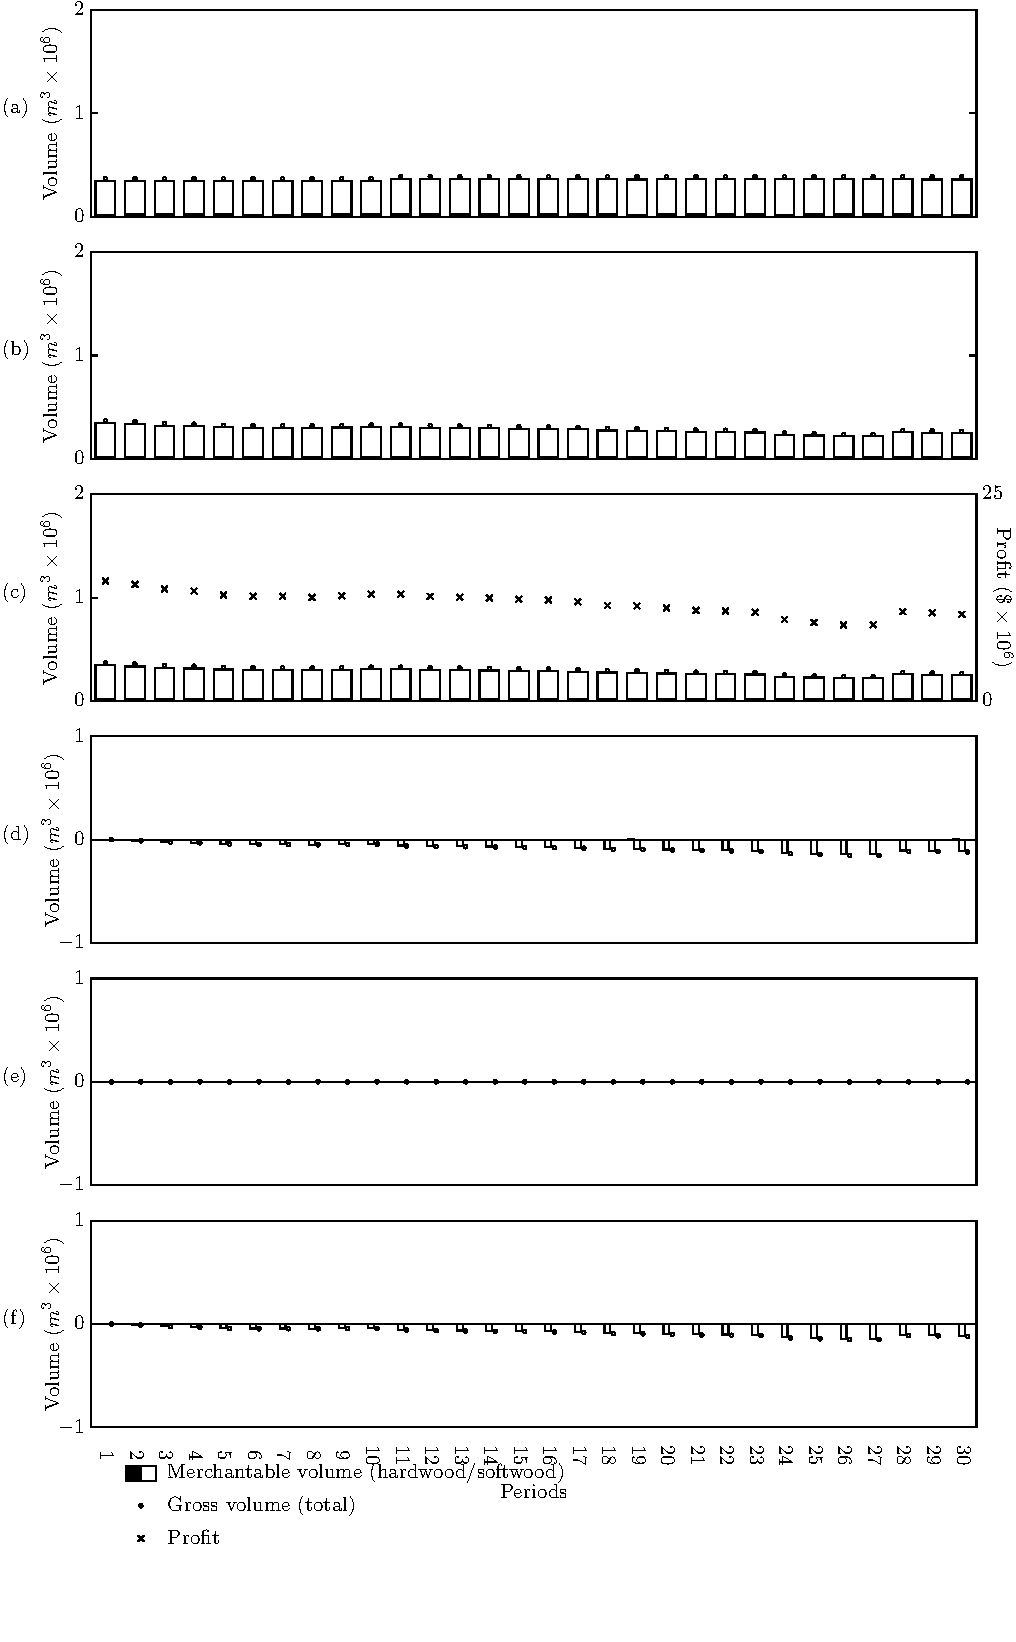
\includegraphics[width=10cm]{images/appendix/s6-1_p30a01}
  \caption{Scenario 6-2y\_f1.0}
  \label{fig:s6-2y_test100}
\end{figure}


\begin{figure}[h]
  \centering
  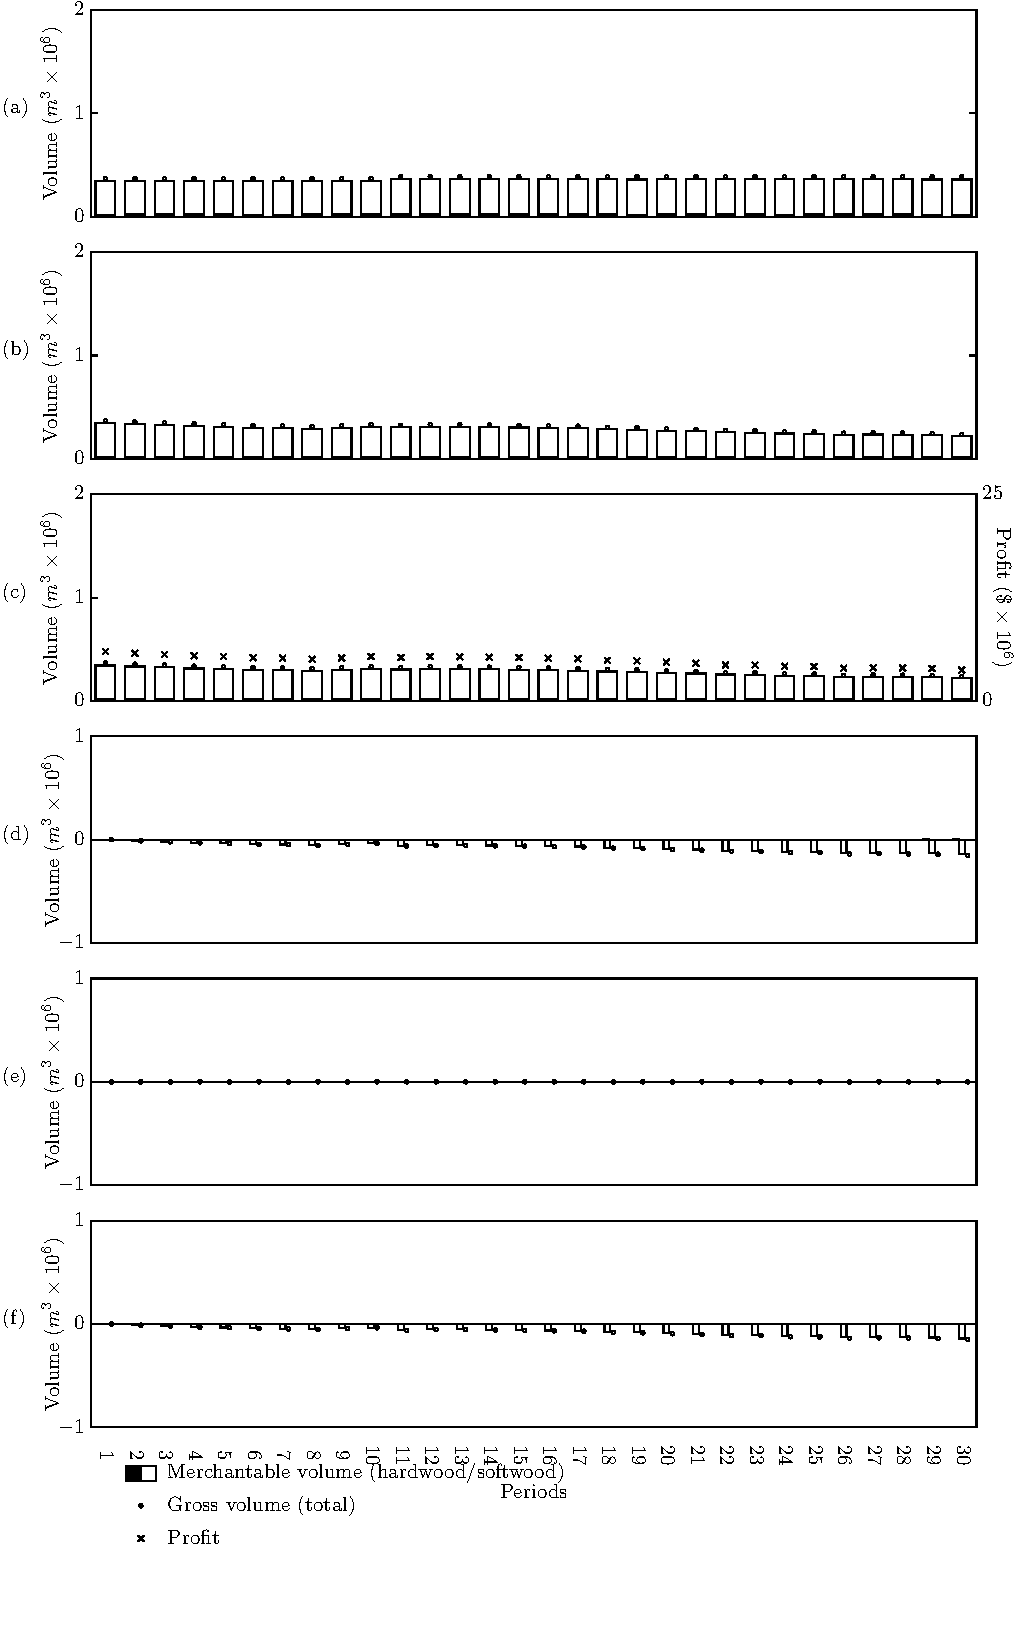
\includegraphics[width=10cm]{images/appendix/s6-2y_test090}
  \caption{Scenario 6-2y\_f6.4}
  \label{fig:s6-2y_test090}
\end{figure}

\begin{figure}[h]
  \centering
  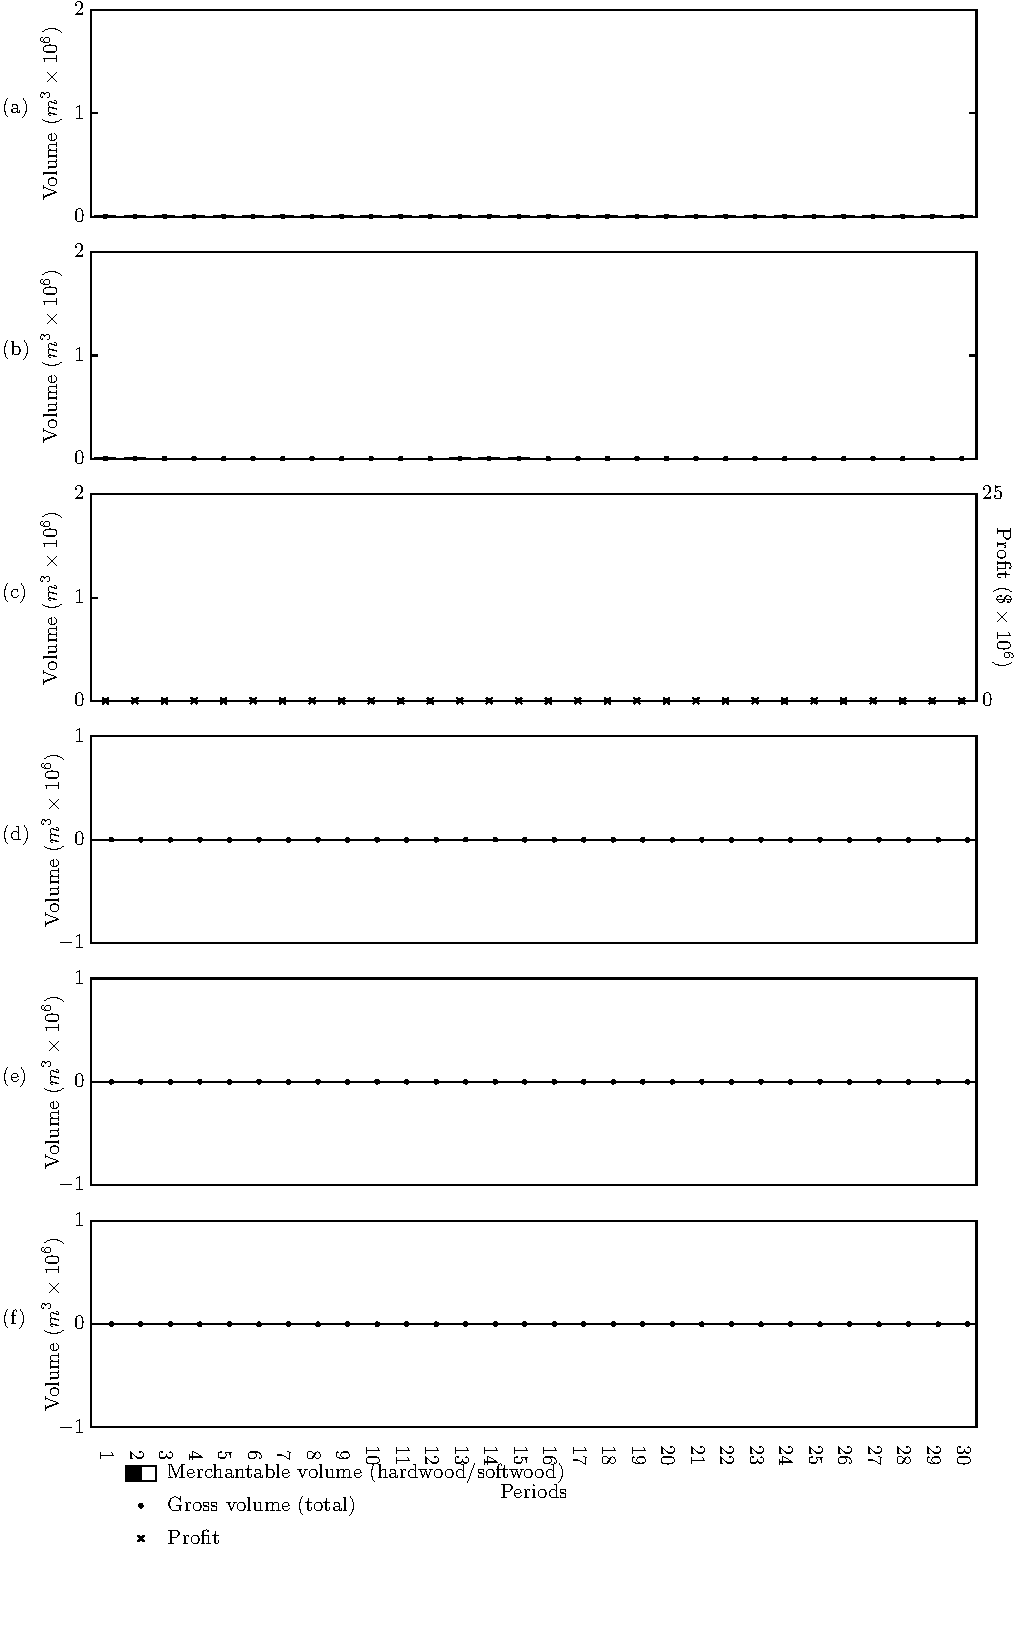
\includegraphics[width=10cm]{images/appendix/s6-2y_test085}
  \caption{Scenario 6-2y\_f0.85}
  \label{fig:s6-2y_test085}
\end{figure}

% \begin{figure}[h]
%   \centering
%   \includegraphics[width=10cm]{images/appendix/s6-2y_test70}
%   \caption{Scenario 6-2y\_f5.3}
%   \label{fig:s6-2y_test70}
% \end{figure}

% \begin{figure}[h]
%   \centering
%   \includegraphics[width=10cm]{images/appendix/s6-2y_test50}
%   \caption{Scenario 6-2y\_f4.0}
%   \label{fig:s6-2y_test50}
% \end{figure}

% \begin{figure}[h]
%   \centering
%   \includegraphics[width=10cm]{images/appendix/s6-2y_test40}
%   \caption{Scenario 6-2y\_f3.4}
%   \label{fig:s6-2y_test40}
% \end{figure}

% \begin{figure}[h]
%   \centering
%   \includegraphics[width=10cm]{images/appendix/s6-2y_test30}
%   \caption{Scenario 6-2y\_f2.8}
%   \label{fig:s6-2y_test30}
% \end{figure}

% \begin{figure}[h]
%   \centering
%   \includegraphics[width=10cm]{images/appendix/s6-2y_test20}
%   \caption{Scenario 6-2y\_f2.2}
%   \label{fig:s6-2y_test20}
% \end{figure}

% \begin{figure}[h]
%   \centering
%   \includegraphics[width=10cm]{images/appendix/s6-2y_test10}
%   \caption{Scenario 6-2y\_f1.6}
%   \label{fig:s6-2y_test10}
% \end{figure}
